\section{Einrichtung und Entwicklung des ``GReQL Converters''}\label{sec:greql-converter}

Der \gls{GReQL Converter} stellt eine Webanwendung dar, die es ermöglicht, GReQL-Regeln aus einem UML-Klassendiagramm zu
extrahieren, das mithilfe von PlantText erstellt wurde. Diese extrahierten Regeln dienen anschließend der Bewertung
von UML-Klassendiagrammen auf der JACK-Plattform. Die Realisierung dieser Anwendung erfolgte mit dem Vue.js-Framework
im Frontend und Node.js im Backend, wie in fig-~\ref{fig:infrastructure} veranschaulicht. In diesem Kapitel wird der
Implementierungsprozess der Plattform sowie ihrer verschiedenen Komponenten ausführlich erläutert.

\begin{figure}[h!]
    \centering
    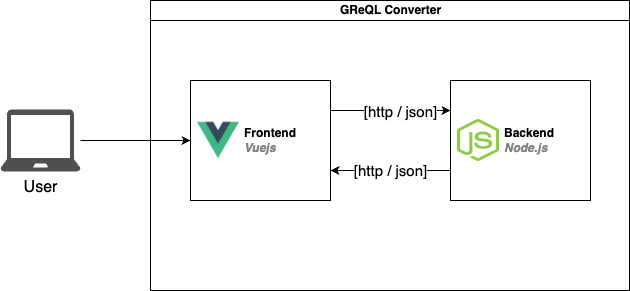
\includegraphics[width=13cm]{images/infrastucture}
    \caption{GReQL-Converter global infrastructure}
    \label{fig:infrastructure}
\end{figure}

\subsection{Einrichtung des PlantUML-Parsers}\label{subsec:einrichtung-des-plantuml-parsers}

Der erste Entwicklungsschritt ist die Konfiguration des PlantUML-parsers. Das ursprüngliche Ziel bestand
darin, eine Anwendung zu entwickeln, die in der Lage ist, PlantText-Code als Eingabe zu akzeptieren und als Ausgabe ein
JSON zu generieren, welches später zur Modellierung von Regelobjekten verwendet werden könnte. Ursprünglich war geplant,
den Parser direkt im Frontend einzusetzen. Es stellte sich jedoch heraus, dass der Parser nur in einer Serverumgebung
effektiv funktioniert. An dieser Stelle gab es zwei Optionen zur Auswahl: die Verwendung eines Tomcat-Servers mit Java
oder eines Node.js-Servers mit JavaScript. Die zweite Option erwies sich als die geeignetere Wahl, da sie es ermöglichte,
dieselbe Programmiersprache für das gesamte Projekt beizubehalten und die Gesamtarchitektur des Systems, einschließlich
seiner zukünftigen Bereitstellung, zu vereinfachen. Node.js eignet sich besonders gut für kleinere Projekte wie dieses.

Im Großen und Ganzen wurde Node.js ausschließlich für die Bereitstellung des Parsers genutzt, was den Backend-Code
erheblich vereinfachte (siehe Code~\ref{lst:bakcend}). Dies ermöglichte einen reibungslosen Übergang zum nächsten Schritt, nämlich
der Erstellung des Grunddesigns der Anwendung.

\subsection{Erstellung des Grunddesigns der Anwendung}\label{subsec:erstellung-des-grunddesigns-der-anwendung}

Um die Ziele des \gls{GReQL Converter}s zu erreichen, ist es von entscheidender Bedeutung, den Benutzern eine elegante,
intuitive und benutzerfreundliche grafische Benutzeroberfläche zur Verfügung zu stellen. Die möglichen Aktionen müssen
auf den ersten Blick leicht erkennbar sein, um das Verständnis zu fördern und dem Benutzer eine schnelle und effiziente
Arbeit zu ermöglichen~\cite{guntupalli2008user}. Die Seite ``Class Converter'' stellt die Benutzeroberfläche dar, auf
der der Benutzer seinen PlantText-Code in GReQL-Code umwandeln kann. Diese Seite ist in drei Hauptabschnitte unterteilt:

\begin{figure}[h]
    \centering
    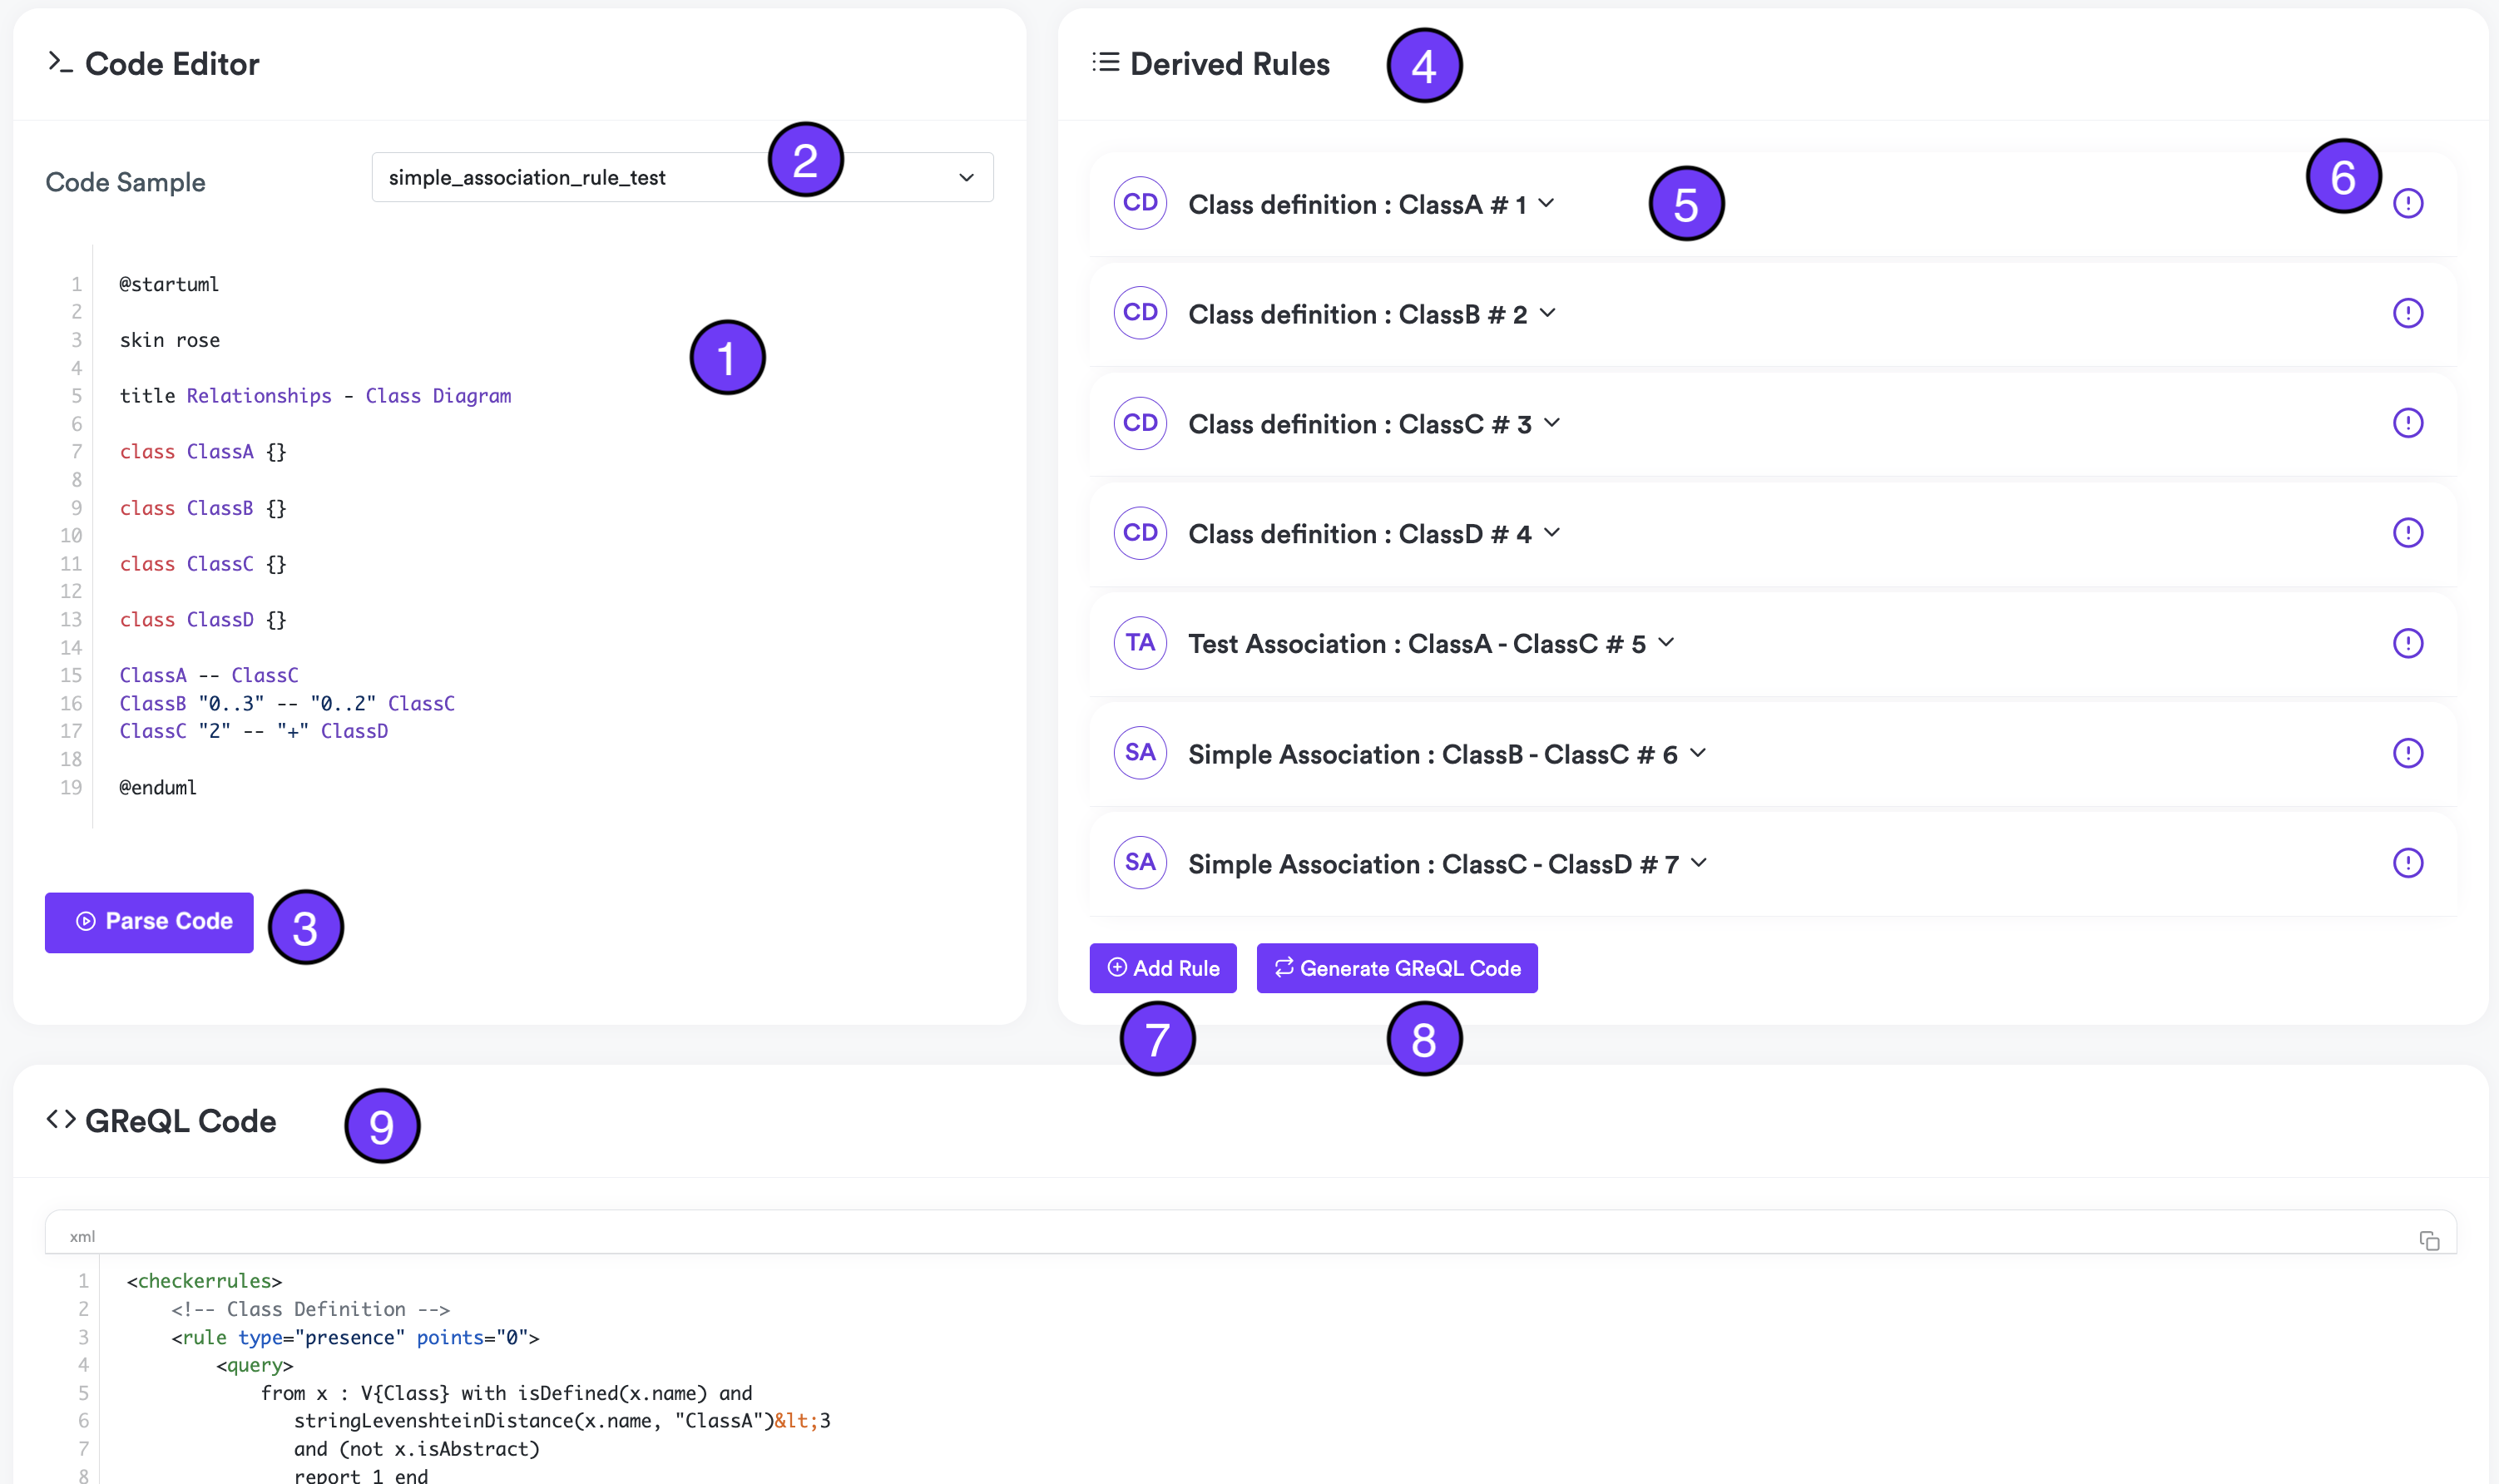
\includegraphics[width=13cm]{images/board}
    \caption{Dashboard im Überblick}
    \label{fig:dashboard}
\end{figure}

\subsubsection{Teil 1: Code editor}

Dieser Abschnitt der grafischen Benutzeroberfläche ist für die Eingabe des PlantUML-Codes durch den Benutzer vorgesehen.
Nachdem der Benutzer die Musterlösung in PlantText modelliert hat, muss er den generierten Code kopieren und in den
Editor einfügen, der durch die Nummer 1 (siehe Abbildung~\ref{fig:dashboard}) gekennzeichnet ist. Darüber hinaus hat der Benutzer die
Möglichkeit, Beispielscodes auszuwählen, wie dies in PlantText der Fall ist und in der Abbildung unter Nummer 2 (siehe Abbildung~\ref{fig:dashboard})
dargestellt ist. Da der geschriebene Code jedoch der in der Dokumentation definierten Struktur entsprechen muss, sind
diese Beispielscodes für den Benutzer nützlich, da sie funktionierende Codebeispiele liefern, von denen er sich
inspirieren lassen und seinen eigenen Code schreiben kann, um die Plattform zu testen. Schließlich ermöglicht der
Button ``Parse Code'' (Nummer 3 - siehe Abbildung~\ref{fig:dashboard}) das Extrahieren der Regelobjekte aus dem Code, was uns zum
Teil 2 führt.

\subsubsection{Teil 2: Derived Rules}

Nachdem der Benutzer auf den Button ``Parse Code'' geklickt hat, wird eine Reihe von Regelobjekten
(Nummer 4 - siehe Abbildung~\ref{fig:dashboard}) aus dem im Code-Editor vorhandenen Code generiert. Diese Regeln werden durch ein
Symbol und einen Titel dargestellt, was es ermöglicht, sie schnell zu unterscheiden und zu identifizieren. Ganz rechts
neben dem Regelobjekt befindet sich ein Ausrufezeichen, das tatsächlich ein Button ist (Nummer 6 - siehe Abbildung~\ref{fig:dashboard}).
Wenn auf diesen Button geklickt wird, öffnet sich eine Dokumentation, die erklärt, was die Regel ist und wie sie
verwendet wird. Wenn der Benutzer auf die Regel klickt (Nummer 5 - siehe Abbildung~\ref{fig:dashboard}), öffnet sich ein Menü,
das es ihm ermöglicht, die in der Regel vorhandenen Informationen nach Belieben zu ändern (siehe Abbildung~\ref{fig:rule_exemple}),
wodurch der \gls{GReQL Converter} zu einem halbautomatischen Werkzeug wird. Diese Informationen variieren je nach Art der Regel
und den für die Generierung des GReQL-Codes erforderlichen Informationen.

\begin{figure}[h!]
    \centering
    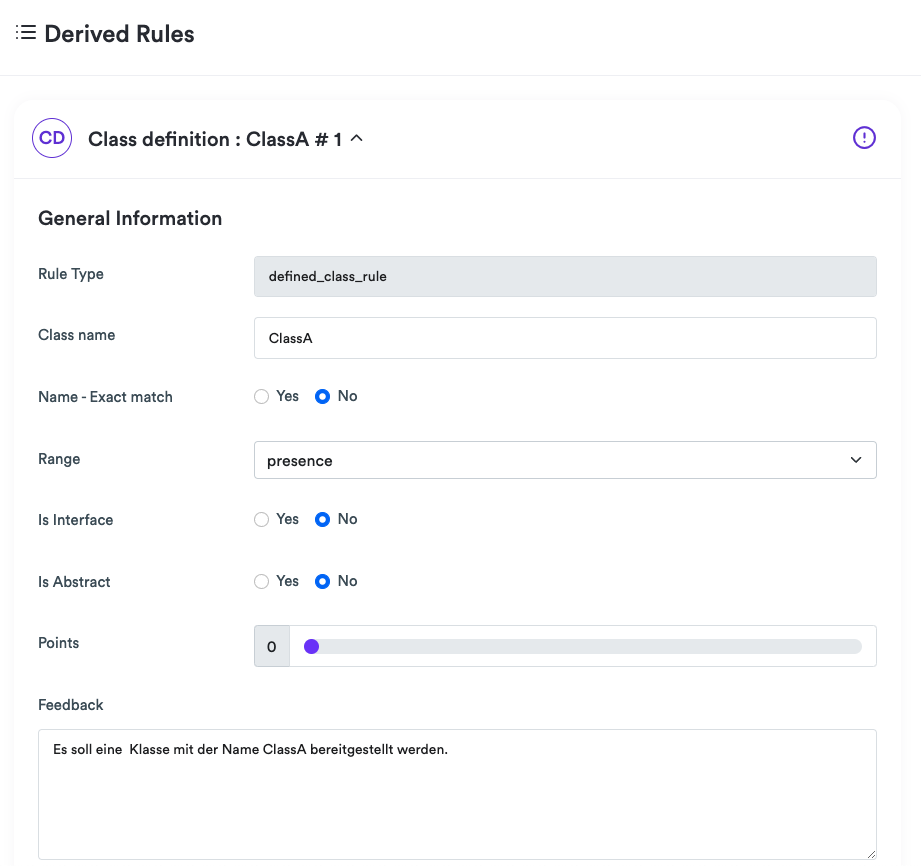
\includegraphics[width=13cm]{images/derived_rule}
    \caption{Beispiel eines Regelobjekts}
    \label{fig:rule_exemple}
\end{figure}

Dann gibt es der Button ``Add Rule'' (Nummer 7 - siehe Abbildung~\ref{fig:dashboard}), die es dem Benutzer ermöglicht,
zusätzliche Regeln hinzuzufügen. Nachdem die Konfiguration und die Änderungen abgeschlossen sind, kann der Benutzer den
GReQL-Code generieren, indem er auf den Button ``Generate GReQL Code'' klickt (Nummer 8 - siehe Abbildung~\ref{fig:dashboard}).
Der GReQL-Code wird aus den zuvor vom Benutzer konfigurierten Regelobjekten generiert.

\subsubsection{Teil 3: GReQL Editor}

Genau wie der erste Abschnitt ist dieser Bereich auch ein Code-Editor, jedoch für XML, da der GReQL-Code im XMI-Format
vorliegt (das auf XML basiert). Dieser Editor (Nummer 9 - siehe Abbildung~\ref{fig:dashboard}) ermöglicht es erfahrenen
Benutzern, die bereits Erfahrung mit GReQL haben, detaillierte und fortgeschrittene Änderungen am generierten Code
vorzunehmen. Auf diese Weise können sie die Abfragen verbessern und spezifizieren, wenn sie sie zu allgemein finden,
oder sie einfach anpassen, je nachdem, was sie im UML-Diagramm bewerten möchten.

Diese drei verschiedenen Teile bilden das grundlegende Design des \gls{GReQL Converter}s. Es gibt auch andere Seiten wie die
Dokumentation oder die Startseite, die nicht erwähnt wurden, da sie in der weiteren Entwicklung keine wesentliche Rolle
spielen. Dieses Design bietet jedoch die Möglichkeit zur Erweiterung, um die Hinzufügung weiterer Seiten und sogar
weiterer Parser zu erleichtern. Der nächste Abschnitt konzentriert sich auf den Prozess der Extraktion von Regelobjekten
aus dem zuvor geparsten Code.

\subsection{Regel-Extraktionsprozess}\label{subsec:regel-extraktionsprozess}


Um den Extraktionsprozess, der in diesem Kapitel beschrieben wird, einzuführen, wird mit einem Beispiel aus der
Modellierung in PlantText angefangen. Die Schritte bis zur Erstellung der Regeln werden verfolgt. Hierzu wird der
folgende PlantText-Code verwendet, der ein UML-Diagramm modelliert (siehe Abbildung~\ref{fig:code-uml}).

\begin{figure}[h!]
    \centering
    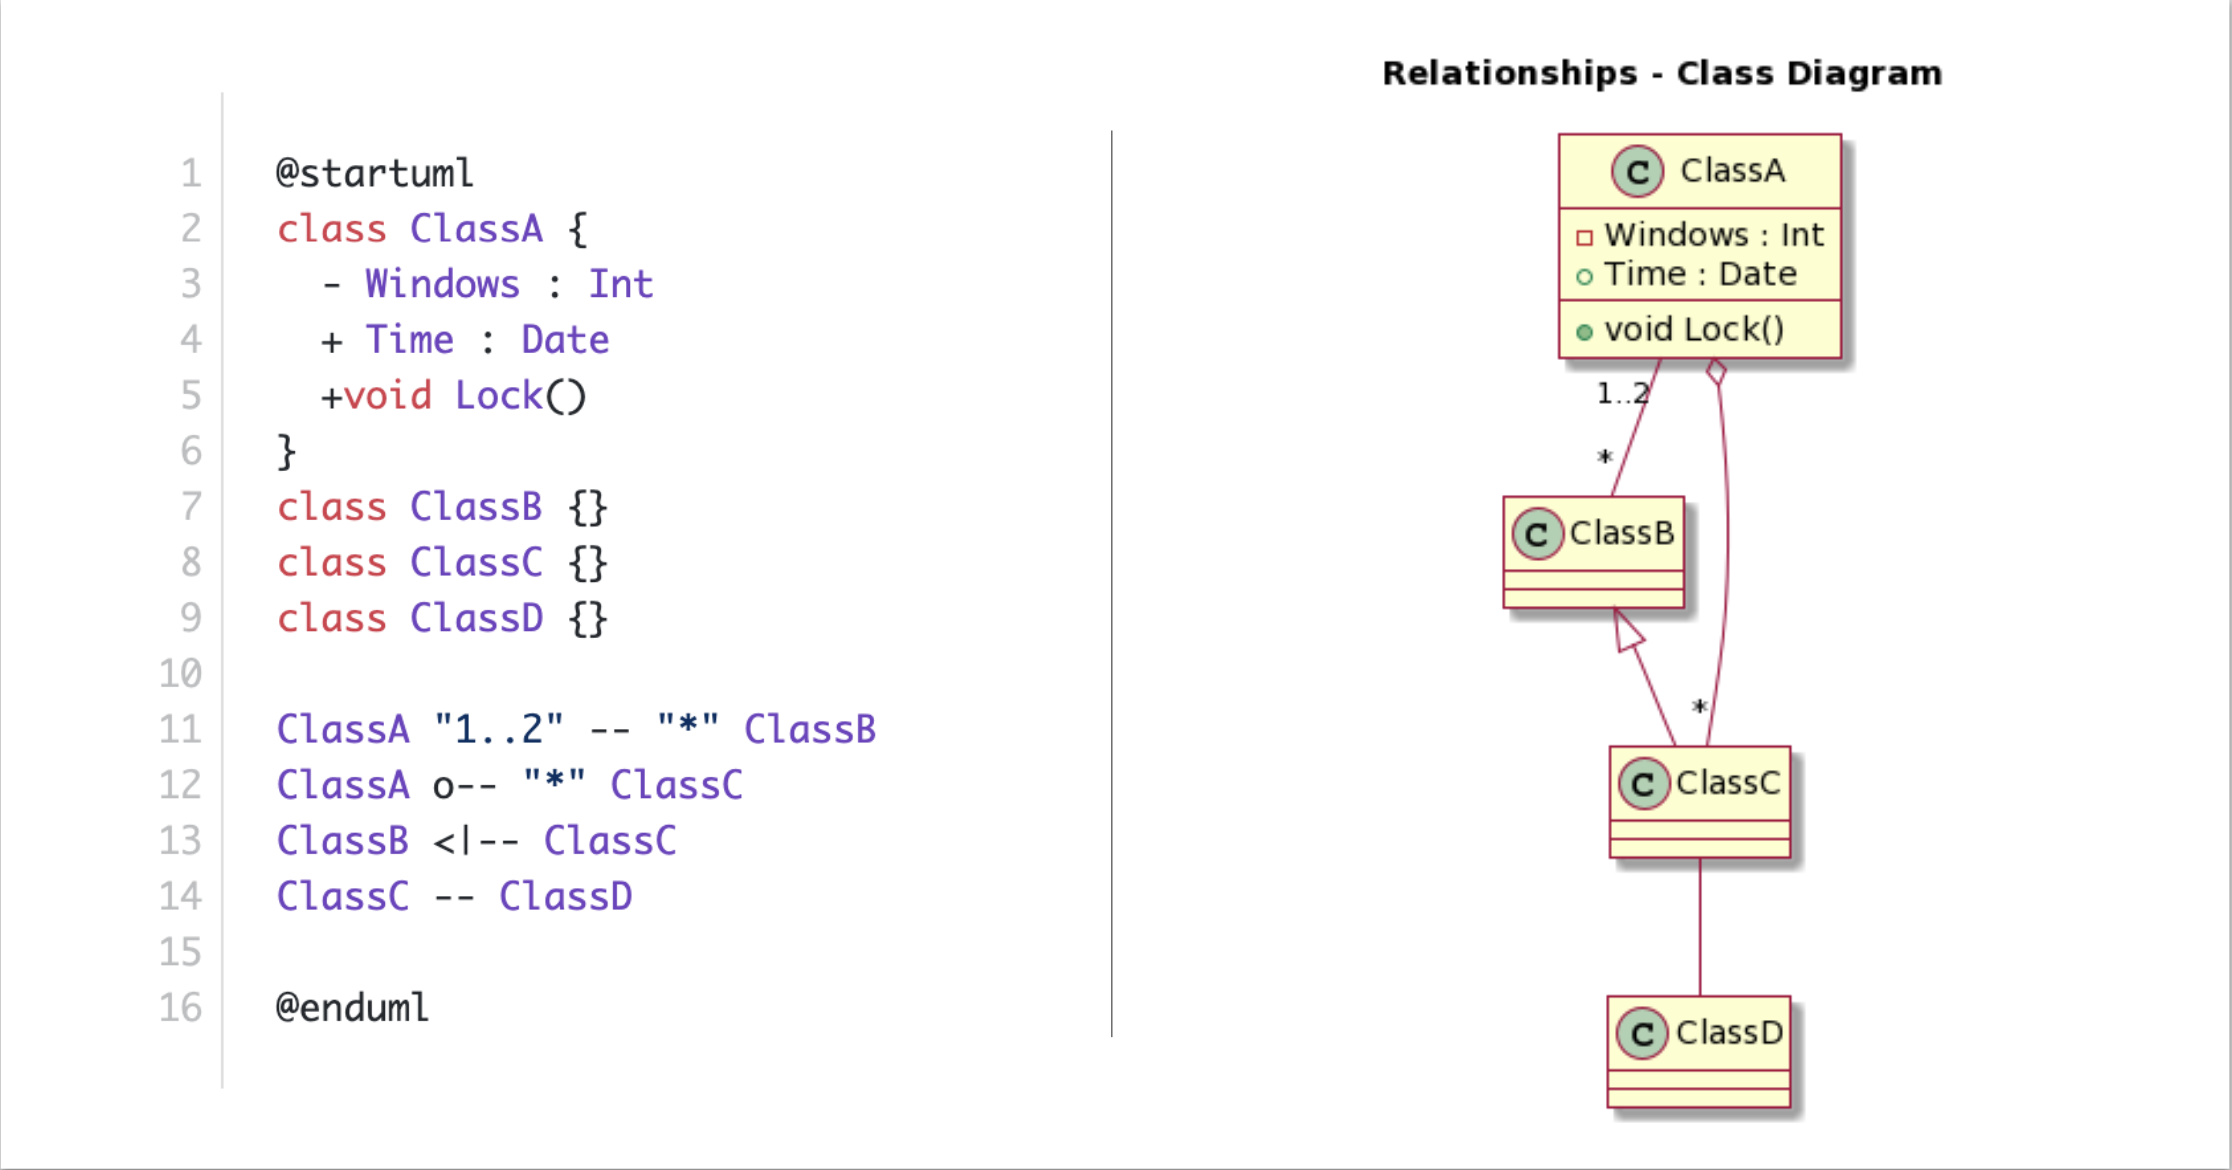
\includegraphics[width=13cm]{images/code-uml}
    \caption{PlantText-Code mit der grafischen Darstellung}
    \label{fig:code-uml}
\end{figure}

Das Diagramm enthält vier Klassen: ClassA, ClassB, ClassC und ClassD\@. ClassA hat drei Elemente: ein privates Attribut
namens ``Windows'' vom Typ Integer (Int), ein öffentliches Attribut namens ``Time'' vom Typ Date und eine öffentliche
Methode namens ``Lock'' ohne Parameter und mit dem Rückgabetyp ``void''. ClassB und ClassC sind leere Klassen ohne
definierte Attribute oder Methoden. ClassD ist ebenfalls eine leere Klasse. Im Diagramm sind verschiedene Beziehungen
zwischen diesen Klassen dargestellt:

\begin{enumerate}
    \item Es gibt eine Assoziationsbeziehung zwischen ClassA und ClassB mit einer Multiplizität von ``1..2'' auf der
Seite von ClassA und einer Multiplizität von ``*'' auf der Seite von ClassB, was bedeutet, dass eine Instanz von ClassA
mit 1 bis 2 Instanzen von ClassB verknüpft ist.
    \item Es besteht eine Kompositionsbeziehung zwischen ClassA und ClassC, die durch ein Rautensymbol auf der Seite von
ClassA gekennzeichnet ist, mit einer Multiplizität von ``*'' auf der Seite von ClassC. Diese Komposition zeigt an, dass
ClassA eine Sammlung von Instanzen von ClassC besitzt und dass diese Instanzen von ClassC von den Instanzen von ClassA
verwaltet werden.
    \item Eine Vererbungsbeziehung (oder Generalisierung) ist zwischen ClassB und ClassC etabliert, gekennzeichnet durch
einen Pfeil, der von ClassC auf ClassB zeigt, mit einer gestrichelten Linie. Dies bedeutet, dass ClassC eine Unterklasse
von ClassB ist, was auf eine Vererbungsbeziehung hinweist.
    \item Schließlich gibt es eine einfache Assoziationsbeziehung zwischen ClassC und ClassD, dargestellt durch eine
durchgehende Linie, was darauf hinweist, dass es eine Verbindung zwischen den beiden Klassen gibt, obwohl die Details
dieser Assoziation im Diagramm nicht spezifiziert sind.
\end{enumerate}


Dies ist eine Darstellung des PlantText-Codes. Sobald dieser Code im \gls{GReQL Converter} vorliegt und der Benutzer auf
``Parse Code'' klickt (Nummer 5 siehe Abbildung~\ref{fig:dashboard}), wird dieser Code über das HTTP-Protokoll an den
Node.js-Server gesendet. Der Server ist dafür verantwortlich, den Code zu analysieren, parsen und ein JSON-Objekt
zurückzugeben, ähnlich dem unten dargestellten:

\begin{lstlisting}[caption={Snippet des JSON-Codes, der nach dem Parsen des PlantText-Codes durch den Server erhalten
wurde.}, label={lst:parsed-json}, language=text]
[
  {
    "elements": [
      {
        "name": "ClassA",
        "title": "ClassA",
        "isAbstract": false,
        "members": [
          {
            "name": "Windows",
            "isStatic": false,
            "accessor": "-",
            "type": "Int"
          },
          {
            "name": "Time",
            "isStatic": false,
            "accessor": "+",
            "type": "Date"
          },
          {
            "name": "Lock",
            "isStatic": false,
            "accessor": "+",
            "returnType": "void",
            "_arguments": ""
          }
        ],
        ...
      },
      ...
      {
        "left": "ClassA",
        "right": "ClassB",
        "leftType": "Unknown",
        "rightType": "Unknown",
        "leftArrowHead": "",
        "rightArrowHead": "",
        "leftArrowBody": "-",
        "rightArrowBody": "-",
        "leftCardinality": "1..2",
        "rightCardinality": "*",
        "label": "",
        "hidden": false
      },
      ...
      {
        "left": "ClassC",
        "right": "ClassD",
        "leftType": "Unknown",
        "rightType": "Unknown",
        "leftArrowHead": "",
        "rightArrowHead": "",
        "leftArrowBody": "-",
        "rightArrowBody": "-",
        "leftCardinality": "",
        "rightCardinality": "",
        "label": "",
        "hidden": false
      }
    ]
  }
]
\end{lstlisting}

Nach Erhalt des JSON wird der Regelgenerierungsprozess gestartet. Basierend auf dem JSON kann für jedes Element eine
zugehörige Regel identifiziert werden. Zum Beispiel, um eine Generalisierung (Vererbung) zwischen zwei Klassen zu
erkennen, reicht es aus, ein Objekt aus dem JSON (hier als ``elem'' bezeichnet) zu betrachten und zu überprüfen, ob
folgende Bedingung erfüllt ist:

\begin{lstlisting}[caption={Evaluationsbedingung für eine Generalisierung}, label={lst:condition-check}, language=javascript]
elem.leftArrowHead.includes("<|") &&
elem.leftArrowBody.includes("-") &&
elem.rightArrowBody.includes("-")
\end{lstlisting}

Dies gilt auch für alle anderen Regeln, die anhand des generierten JSON identifiziert werden können. Einige
UML-Feinheiten werden jedoch nicht vom Parser erkannt, was in einem späteren Abschnitt erläutert wird. Bei der
Entwicklung des GReQL Converters wurden eine Reihe von Regeln definiert, darunter:

\subsubsection{Class definition}
Diese Regel hat zum Ziel, die Anwesenheit oder Abwesenheit einer Klasse in einem UML-Diagramm zu bestimmen. Darüber
hinaus ermöglicht sie die Extraktion verschiedener Merkmale dieser Klasse. Mit Hilfe dieser Regel können Informationen
wie die Abstraktion der Klasse, ihre Interface-Natur, die Methoden (einschließlich der Parameter und des Rückgabetyps),
die Attribute und ihre Typen extrahiert werden (siehe Code~\ref{lst:rules_def}). Nach Extraktion dieser Informationen wird
ein entsprechendes JSON-Objekt erstellt und einer Liste von Objekten hinzugefügt.

\subsubsection{Enum definition}
Das Ziel dieser Regel besteht darin, Enumerationen in einem UML-Diagramm zu identifizieren. Nachdem eine Enumeration
ordnungsgemäß identifiziert wurde, geht es darum, alle verschiedenen Attribute zu identifizieren, die sie zusammensetzen,
was ebenfalls in dieser Regel durchgeführt wird (siehe Code~\ref{lst:rules_def}). Nach dieser Identifizierung wird ein
entsprechendes JSON-Objekt erstellt und der Liste von Objekten hinzugefügt.

\subsubsection{Generalization}
Diese Regel dient dazu, die verschiedenen Vererbungsbeziehungen zwischen Klassen und Schnittstellen zu definieren.
Sie wird erstellt, wenn eine Klasse von einer anderen erbt oder eine Schnittstelle implementiert. Die Details dieser
Beziehung werden erkannt, und ein JSON-Objekt wird generiert und zu einer Objektliste hinzugefügt (siehe Code~\ref{lst:rules_def}).

\subsubsection{Simple Association}
Diese Regel zielt darauf ab, die Assoziationsbeziehungen zwischen Klassen mit ihren jeweiligen Vielfachen zu definieren.
Wenn eine Assoziation erkannt wird, werden die Klassennamen und die Vielfachen in einem JSON-Objekt gespeichert, das
anschließend zu einer Objektliste hinzugefügt wird (siehe Code~\ref{lst:rules_def}).

\subsubsection{Composition und Aggregation}
Diese beiden Regeln dienen dazu, die verschiedenen Compositions- und Aggregationsbeziehungen im UML-Diagramm zu
identifizieren und zu definieren. Das generierte Objekt enthält auch Multiplizitäten, die bei der Generierung von
GReQL-Code wichtig sind. Dieses Objekt wird dann zu einer Liste von Objekten hinzugefügt (siehe Code~\ref{lst:rules_def}).

\subsubsection{Association Class}
Diese Regel ermöglicht es, die Beziehung von Assoziationsklassen zu identifizieren und zu definieren. Obwohl sie in den
meisten UML-Diagrammen während der Modellierung selten verwendet wird, spielt sie dennoch bei der Bewertung eine
wichtige Rolle. Das generierte JSON-Objekt enthält im Wesentlichen Informationen zur zugehörigen Klasse und nicht direkt
zur Beziehung (siehe Code~\ref{lst:rules_def}).

\subsubsection{Nomination Consistency (optional)}
Diese Regel dient dazu, festzustellen, ob das zu bewertende Diagramm eine Konsistenz bei der Benennung der verschiedenen
Attribute aufweist. Zum Beispiel gilt es als schlechte Praxis, Attribute gleichzeitig mit Groß- und Kleinbuchstaben zu
benennen~\cite{albert2003implementing}. Ein JSON-Objekt wird generiert und zu einer Liste von Objekten hinzugefügt.
Diese Regel ist optional, was bedeutet, dass sie zu den Regeln gehört, die vom Lehrer selbst hinzugefügt werden müssen.
Sie wird also nicht automatisch generiert (siehe Code~\ref{lst:rules_def}).

\subsubsection{Count Methods (optional)}
Diese Regel ermöglicht es, die Anzahl der im UML-Diagramm vorhandenen Methoden zu definieren. Der Lehrer muss als
Parameter die genaue Anzahl der Methoden angeben, die im UML-Diagramm des Schülers vorhanden sein müssen.
Ein JSON-Objekt wird generiert und zu einer Liste von Objekten hinzugefügt. Diese Regel ist optional, was bedeutet,
dass sie zu den Regeln gehört, die vom Lehrer selbst hinzugefügt werden müssen. Sie wird also nicht automatisch
generiert (siehe Code~\ref{lst:rules_def}).

\subsubsection{Count Attributes (optional)}
Diese Regel ermöglicht es, die Anzahl der im UML-Diagramm vorhandenen Attribute zu definieren. Der Lehrer muss als
Parameter die genaue Anzahl der Attribute angeben, die im UML-Diagramm des Schülers vorhanden sein müssen. Diese Regel
ähnelt der Regel Count Methods (siehe Code~\ref{lst:rules_def}).

\subsubsection{Test Association}
Diese Regel dient einfach dazu, festzustellen, ob es eine Beziehung zwischen zwei Klassen gibt. Ein JSON-Objekt wird
generiert und zu einer Liste von Objekten hinzugefügt (siehe Code~\ref{lst:rules_def}).

\begin{figure}[h!]
    \centering
    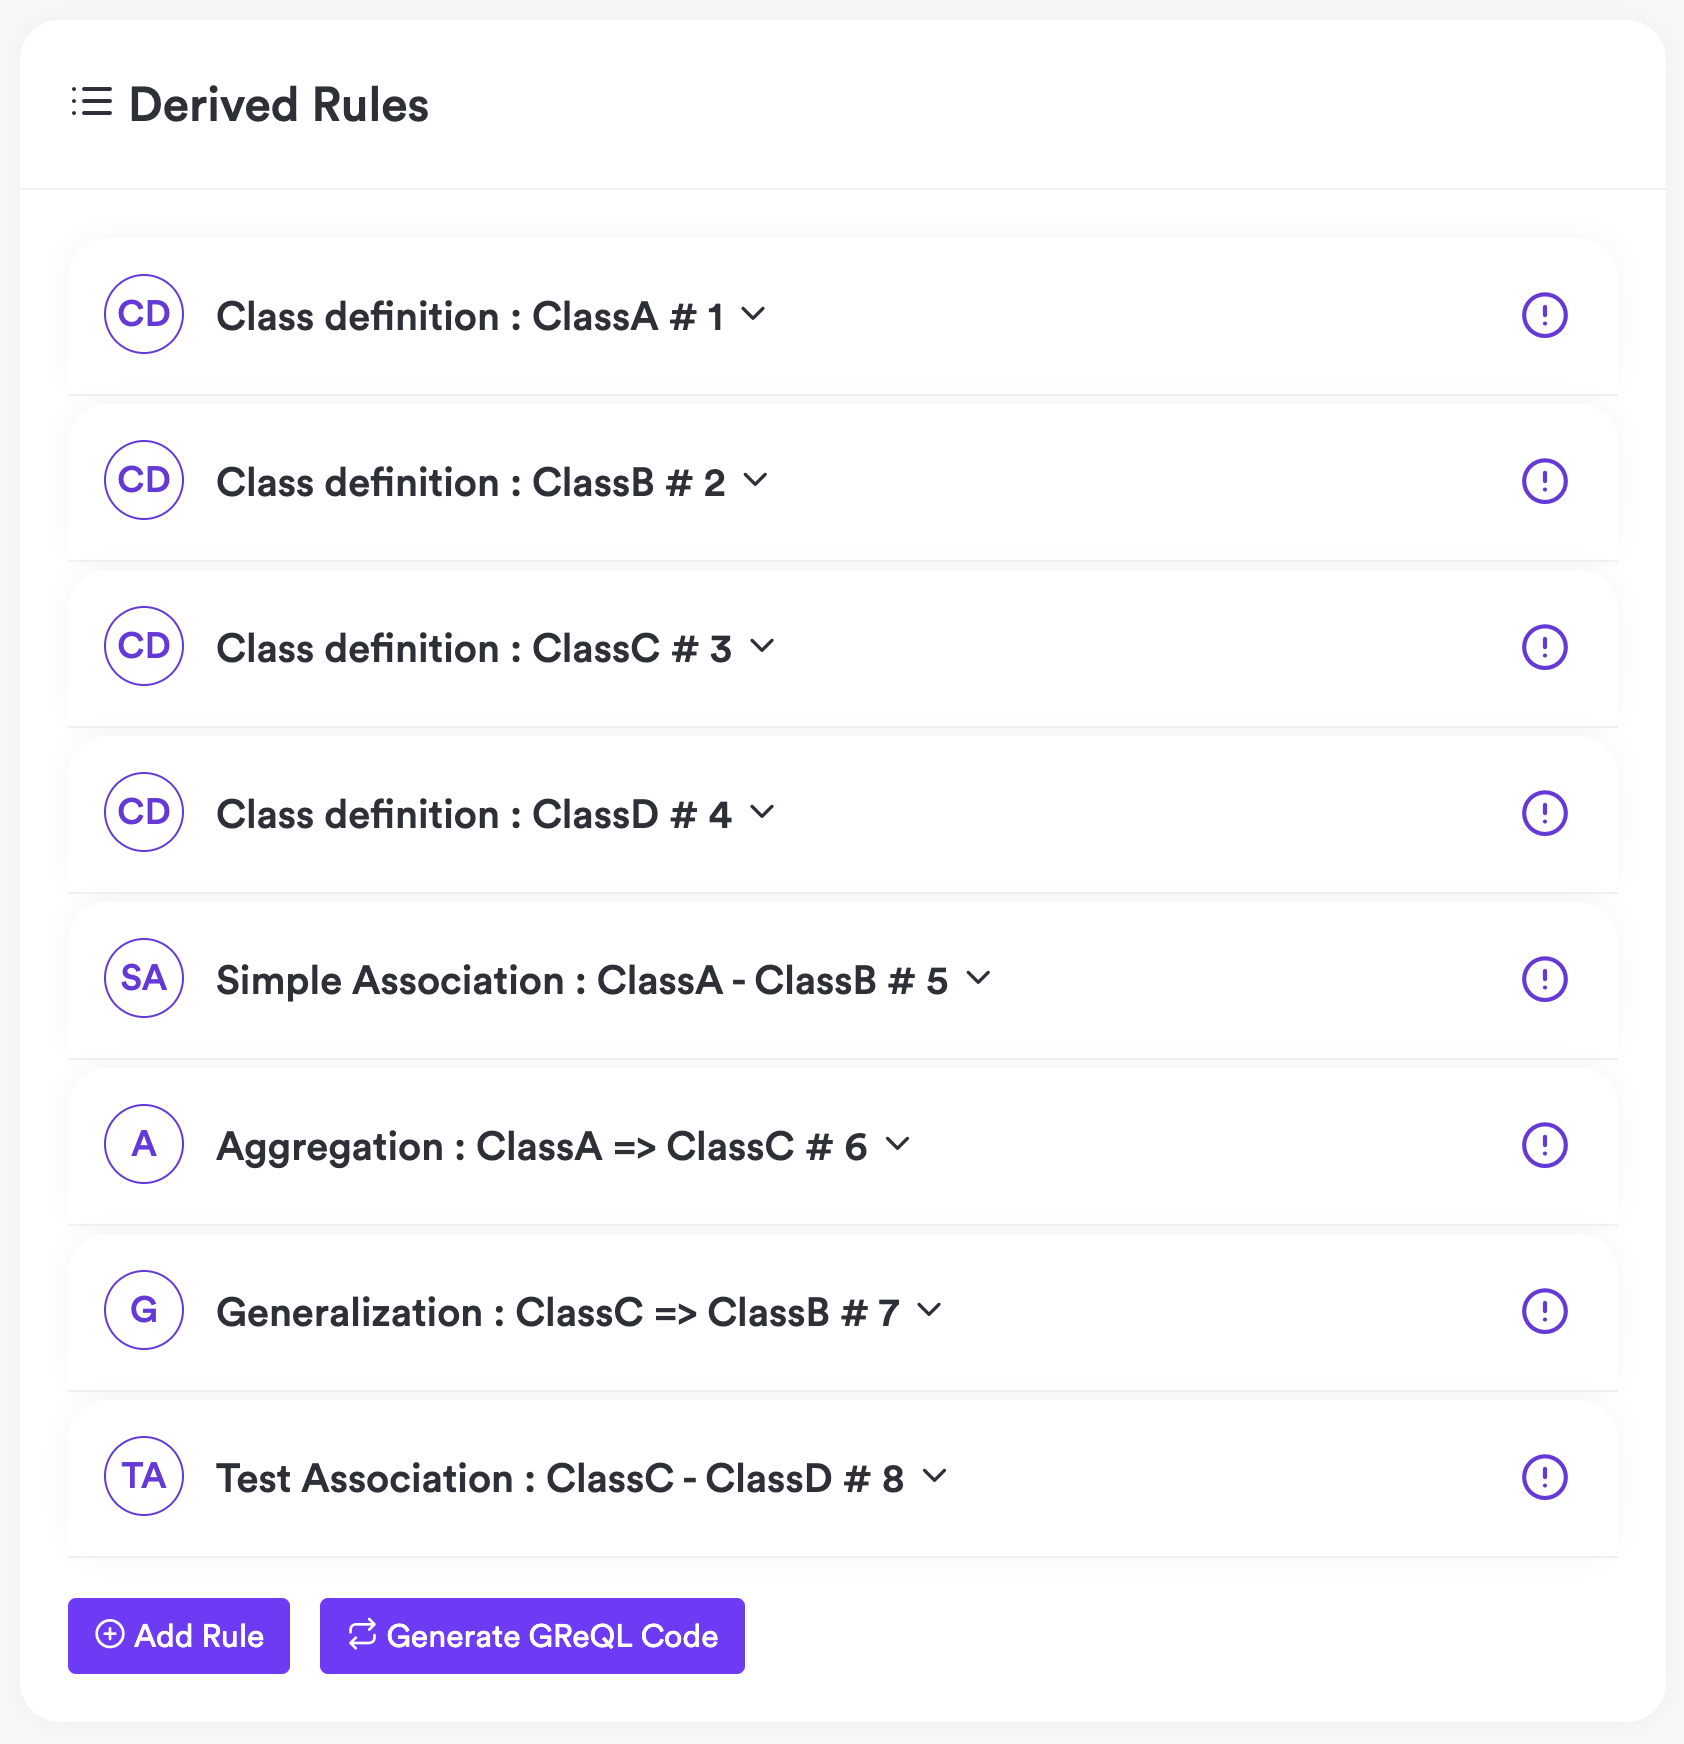
\includegraphics[width=13cm]{images/extracted_rules}
    \caption{Regeln, die dem geparsten PlantText-Code entsprechen}
    \label{fig:extracted_rules}
\end{figure}

\\~\\
Die zuvor erwähnte Objektliste enthält nun alle Regeln, die aus dem vom Node.js-Server bereitgestellten JSON extrahiert
wurden. Jede dieser Regeln wird auf der Frontend-Seite angezeigt und ist anpassbar (siehe Abbildung~\ref{fig:rule_exemple}).
Der Benutzer hat somit die Möglichkeit, jede Regel nach seinen Wünschen anzupassen, indem er beispielsweise Kommentare,
Punkte (Points) sowie jeden mit der jeweiligen Regel verknüpften Attribut ändert. Auf diese Weise werden die Regeln aus dem JSON
extrahiert und angepasst. Anschließend folgt der nächste Schritt, bei dem diese Regeln in GReQL-Code umgewandelt werden.


\subsection{Umwandlung der Regel-Objekte in GReQL-Code}\label{subsec:umwandlung-der-regel-objekte-in-greql-code}
Nach dem Extrahieren und Anpassen der Regeln ist es nun möglich, GReQL-Code aus der Liste zu generieren, die die Objekte
darstellt, welche diese Regeln repräsentieren. Tatsächlich hat jede Regel eine entsprechende Vorlage. Obwohl es
verschiedene Möglichkeiten gibt, GReQL-Code zu schreiben, wurde im Verlauf der Entwicklung nach einer optimierten
Variante gesucht, die das schnellste und effizienteste Ergebnis mit minimalem Code ermöglicht. Konkret geht es darum,
den GReQL-Code so anzupassen, dass er perfekt zur zu konvertierenden Regel passt, und ihn dann als Vorlage zu verwenden.
Zum Beispiel für die Regel, die das Vorhandensein einer Klasse definiert (siehe Code~\ref{lst:class_def_xml}):
\\~\\
\begin{lstlisting}[caption={Class Definition Template \(erster Teil\)}, label={lst:class_def_xml}, language=xml]
<rule type="${rule.existence}" points="${rule.points}">
    <query>
        from x : V{Class}
           with
           isDefined(x.name) and
           stringLevenshteinDistance(x.name,
           "${rule.rule_specific.class_name}")&lt;3
           ${abstractCode}
           report 1 end
    </query>
    <feedback>
        ${rule.feedback}
    </feedback>
</rule>
\end{lstlisting}

Nachdem die Vorlage erhalten wurde, werden die Parameter durch diejenigen aus dem Regelobjekt ersetzt. Auf diese Weise
wird für jedes Objekt eine entsprechende Regel erstellt. Dieser Prozess kann je nach den verschiedenen Regeln und
Objekten variieren, bleibt jedoch im Wesentlichen für die meisten Regeln gleich. Am Ende dieses Prozesses wird einen
gültigen GReQL-Code erhalten, der auf der JACK-Plattform verwendet werden kann.
\\~\\
\begin{lstlisting}[!h, caption={Ausschnitt aus dem GReQL-Code, der nach der Konvertierung erhalten wurde}, label={lst:final_xml_convert}, language=xml]
<checkerrules>
    <!-- Class Definition -->
    <rule type="presence" points="0">
        <query>
            from x : V{Class} with isDefined(x.name) and
               stringLevenshteinDistance(x.name,
               "ClassA")&lt;3
               and (not x.isAbstract)
               report 1 end
        </query>
        <feedback>
            Es soll eine Klasse mit der Name
            ClassA bereitgestellt werden.
        </feedback>
    </rule>
    <!-- Class Definition -->
    <rule type="presence" points="0">
        <query>
            from x : V{Class} with
               isDefined(x.name) and
               stringLevenshteinDistance(x.name,
               "ClassB")&lt;3
               and (not x.isAbstract)
               report 1 end
        </query>
        <feedback>
            Es soll eine Klasse mit der Name
            ClassB bereitgestellt werden.
        </feedback>
    </rule>

    ...

    <!-- Generalization rule -->
    <rule type="presence" points="0">
        <query>
            from a,b : V{Class}
                   with
                      isDefined(a.name) and
                      a.name="ClassC" and
                      isDefined(b.name) and
                      b.name="ClassB" and
                      a --> V{Generalization} --> b
                   report 1 end
        </query>
        <feedback>
            Das Diagramm sollte eine Klasse
            ClassC enthalten, die von einer
            Oberklasse ClassB erbt.
        </feedback>
    </rule>
    <!-- Test Association Rule -->
    <rule type="presence" points="0">
        <query>
            from x,y : V{Class}
                           with
                              isDefined(x.name) and
                              x.name="ClassC" and
                              isDefined(y.name) and
                              y.name="ClassD" and
                              x --> V{Property}
                              --> V{Association}
                              &lt;-- V{Property}
                              &lt;-- y
                           report 1 end
        </query>
        <feedback prefix="Hinweis">
            Im Diagramm gibt es keine directe Association
            zwischen die Klasse "ClassD" und
            die Klasse "ClassC". Das kann durch eine
            bessere Modellierung vermieden werden.
        </feedback>
    </rule>
</checkerrules>
\end{lstlisting}

\section{Entwicklung eines Annotationssystems}
In der in Abschnitt~\ref{sec:darlegung-des-workflow-prozesses} beschriebenen ersten Phase (die das Schreiben des
plantText-Codes in den GReQL Converter umfasst), folgt die zweite Phase, in der die generierten Regelobjekte modifiziert
werden. Es ist jedoch wichtig zu beachten, dass dieser Prozess zur Modifikation der Regelobjekte als äußerst
arbeitsintensiv angesehen werden kann. Um dies zu verdeutlichen, kann das Beispiel der Anpassung der Anzahl der Punkte (Points)
für jede Regel in einem Diagramm mit mehr als zwanzig Regeln dienen. Diese Aufgabe erweist sich schnell als zeitaufwändig,
da jede Regel individuell bearbeitet werden muss, um die erforderlichen Änderungen vorzunehmen. Ebenso stellt sich die
gleiche Problematik ein, wenn es um die Eigenschaft ``Exact match'' (siehe Abbildung~\ref{fig:code-uml}) geht (die festlegt, ob
der Name eines Attributs, einer Methode oder einer Klasse genau mit dem im Diagramm angegebenen Namen übereinstimmen
muss oder ob eine gewisse Fehlermarge akzeptiert wird).

Um diesen Prozess zu erleichtern, wurde im GReQL Converter ein Annotationssystem implementiert. Dieses Vorhaben zielt
zunächst darauf ab, einige Attribute des PlantUML-Parsers zu nutzen, die in Bezug auf UML-Diagramme vergleichsweise
selten verwendet werden, insbesondere Generika, sowie das Labeling-System von PlantText. Hierfür wurde eine spezifische
Syntax entwickelt, deren Einzelheiten in der Dokumentation des GReQL Converters erläutert sind. Das folgende Beispiel~\ref{fig:annotation}
zeigt einen Anwendungsfall dieser Syntax für die Annotation einer Klasse:

\begin{figure}[h!]
    \centering
    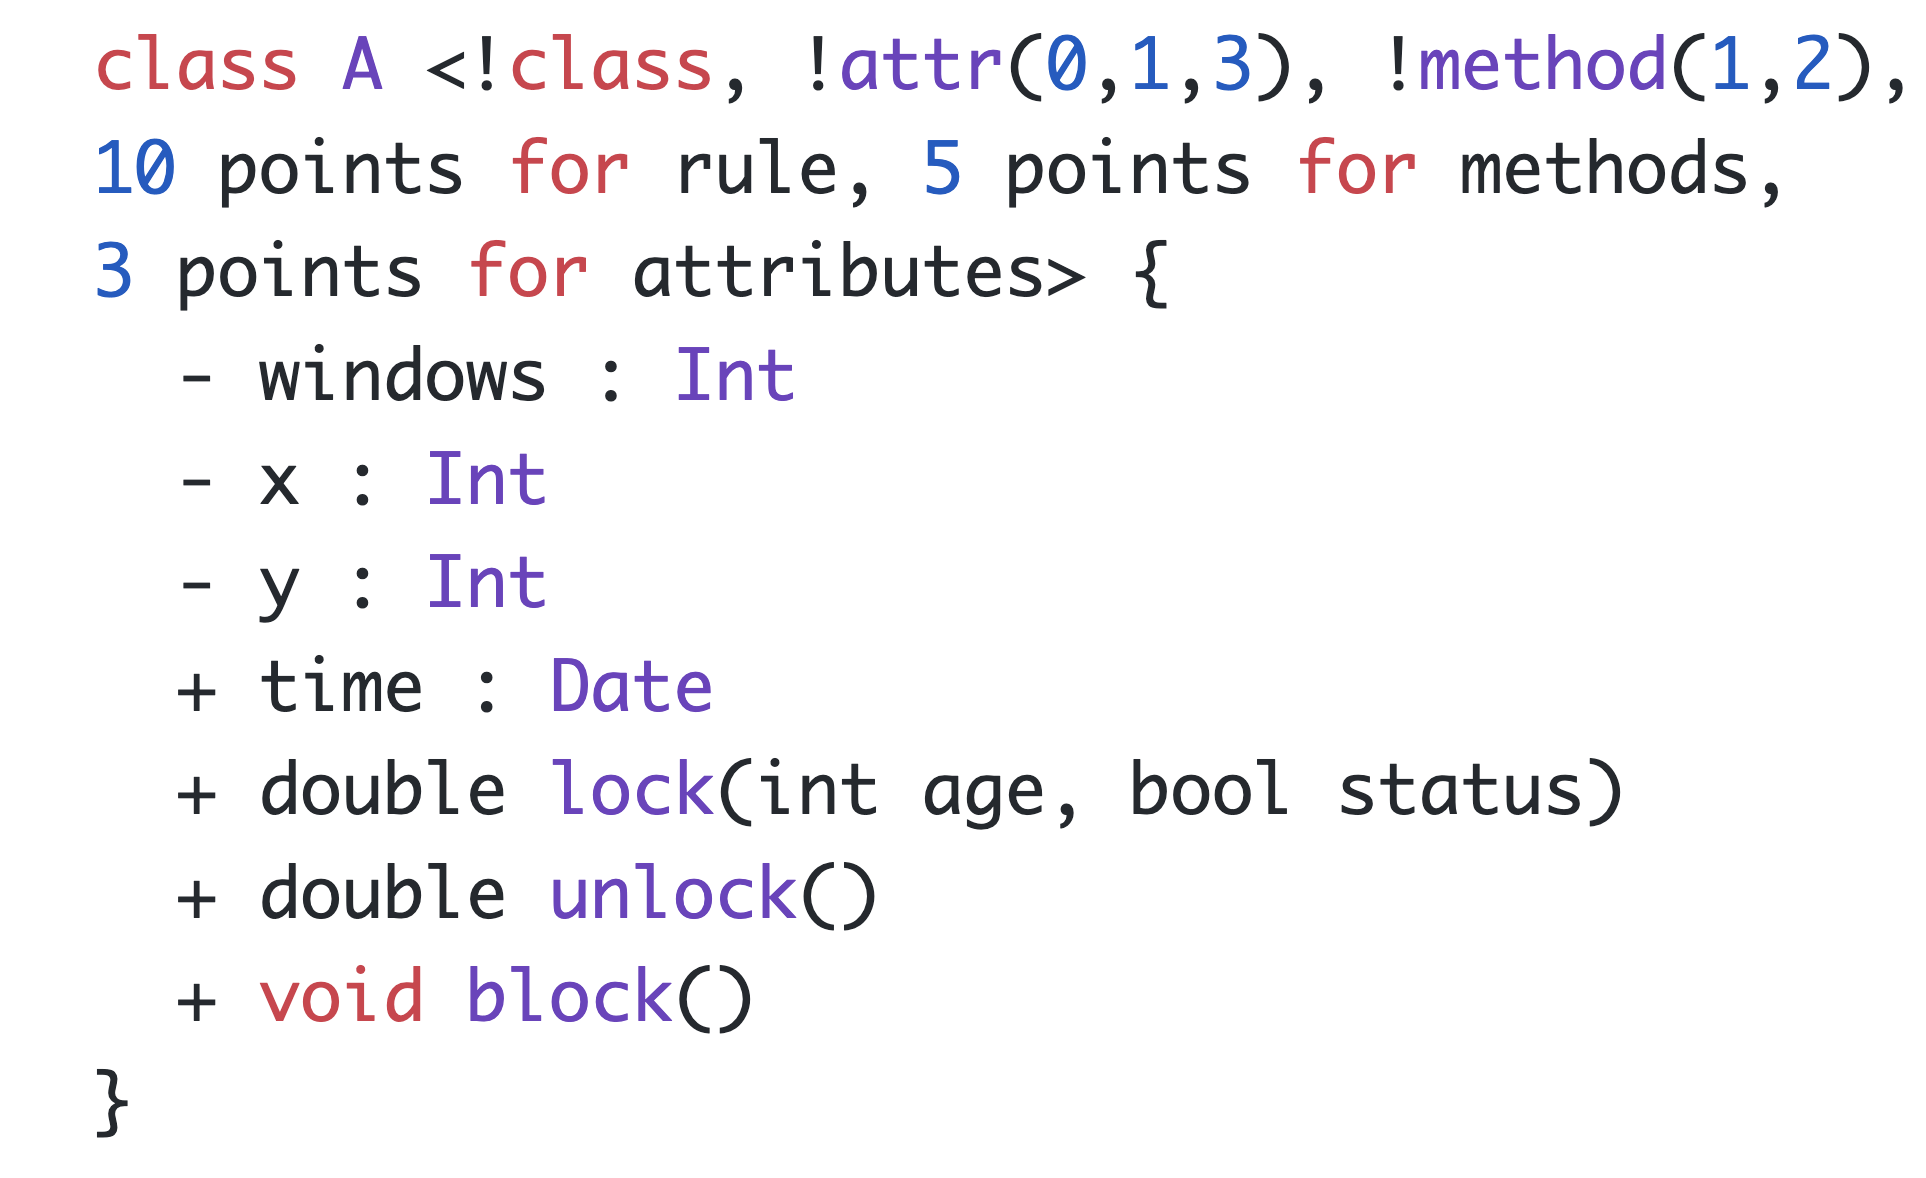
\includegraphics[width=10cm]{images/annotation}
    \caption{Beispiel für die Verwendung des Annotationssystems}
    \label{fig:annotation}
\end{figure}

\begin{itemize}[label={}]
    \item \textbf{!class}: Die Verwendung der Direktive ``!class'' dient dazu, die Funktion der exakten Übereinstimmung
    (Exact match) anhand von Klassennamen zu aktivieren.
    \item \textbf{!attr(0,1,3)}: Die Direktive ``!attr(0,1,3)'' wird verwendet, um die exakte Übereinstimmung (Exact match) in den
    ersten, zweiten und vierten Attributen, nämlich ``windows'', ``x'' und ``time'' zu aktivieren.
    \item \textbf{!attr(*)}: Wenn beabsichtigt wird, die exakte Übereinstimmung (Exact match) in allen Attributen zu aktivieren,
sollte die Direktive ``!attr(*)'' verwendet werden.
    \item \textbf{!method(1,2)}: Die Direktive ``!method(1,2)'' wird verwendet, um die exakte Übereinstimmung (Exact match) in den
zweiten und dritten Methoden, nämlich ``unlock'' und ``block'' zu aktivieren.
    \item \textbf{!method(*)}: Sollte der Wunsch bestehen, die exakte Übereinstimmung (Exact match) in allen Methoden zu
aktivieren, sollte die Direktive ``!method(*)'' verwendet werden.
    \item \textbf{x points for rule}: Bestimmt, wie viele Punkte (X) die Regel der Klassendefinition haben sollte.
    \item \textbf{y points for attributes}:  Bestimmt, wie viele Punkte (Y) die Attributregeln haben sollten.
    \item \textbf{z points for methods}: Bestimmt, wie viele Punkte (Z) die Methodenregeln haben sollten.
\end{itemize}


Ursprünglich wurde in Betracht gezogen, Annotationen direkt vor den relevanten Attributen oder Methoden zu platzieren,
um das Exact Matching auf die Attribute oder Methoden zu aktivieren. Jedoch stellte sich heraus, dass dies nicht
praktikabel war. Jedes Mal, wenn ein Sonderzeichen zur Unterscheidung und Abfrage der gewünschten Informationen
hinzugefügt wurde, löste der PlantUML-Parser einen Fehler aus. Selbst der Versuch, den Namen des Attributs zu
modifizieren, beispielsweise durch ``number*exact'' oder ``number!exact'', erwies sich als nicht funktionsfähig.
Daher wurde beschlossen, auf Klassenebene zu arbeiten, da dies als der zugänglichste Ansatz für die Umsetzung dieser
Funktion erschien. Bisher wurde keine andere Möglichkeit gefunden, diesen Ansatz zu umgehen.

\\~\\
Dieses Annotierungssystem beschleunigt und optimiert signifikant den Prozess der Generierung von GReQL-Code. Sobald
die Beherrschung dieses Annotierungssystems erreicht ist, werden Lehrende nicht länger auf die Zwischenrepräsentation
von Regelobjekten angewiesen sein, da sie in der Lage sein werden, GReQL-Code direkt mit der PlantText-Code und der
Annotation zu generieren.

\section{Erweiterbarkeit des GReQL-Converters}\label{sec:erweiterbarkeit-des-greql-converters}

Der GReQL Converter wurde so entwickelt, dass eine einfache Erweiterung möglich ist. Dies ermöglicht zukünftigen
Entwicklern, die Funktionalität des Tools zu erweitern, ohne mehrere Teile des Codes ändern zu müssen, was zu Fehlern
führen könnte. Dieser Abschnitt präsentiert die Gesamtarchitektur des Datentransits im GReQL Converter sowie
verschiedene Möglichkeiten zur Erweiterung des Tools.

\subsection{Datentransit im GReQL-Converter}\label{subsec:datentransit-im-greql-converter}

Der Prozess zur Generierung des GReQL-Codes aus dem GReQL Converter durchläuft mehrere Schritte, die bereits in diesem
Kapitel beschrieben wurden. Diese Sektion bietet detaillierte Einblicke, die wichtig sind, um zu
verstehen, wie die Funktionalitäten des Tools erweitert werden können. Dieser Prozess wird durch
Abbildung~\ref{fig:transit} veranschaulicht, die die verschiedenen Schritte des Datentransits zeigt.


Es beginnt zunächst mit dem PlantText-Code der Lehrkraft, der an den PlantUML-Parser gesendet wird, der auf einem
Node.js-Server läuft. Der Parser gibt ein JSON-Objekt zurück, das Informationen über die UML-Entitäten sowie deren
Beziehungen enthält (siehe Code~\ref{lst:parsed-json}). Nach diesem Schritt wird dieses JSON vom ``Class Converter''
verarbeitet. Der Class Converter nutzt das JSON des Parsers und enthält Methoden zur Identifizierung von Entitäten und
Beziehungen, wodurch Regeln für jede Entität und Beziehung generiert werden. Die Art und Weise dieser
Identifizierung wird im Implementierungskapitel beschrieben (siehe Code~\ref{lst:condition-check}).


Der Class Converter verwendet die ``Class Rules Definition'' zur Generierung der Regeln. Die Class Rules Definition ist
eine Art Enum, die als Konfigurationsdatei betrachtet werden kann (siehe Code~\ref{lst:rules_def}). Sie enthält alle
Definitionen für jedes Objekt des Regeltyps. In dieser Datei ist es möglich, eine neue Regel und ihre Attribute zu
definieren. Mithilfe dieser Datei kann der Class Converter Regeln basierend auf dem JSON des Parsers generieren.
Die Verwendung der Class Rules Definition spielt eine entscheidende Rolle im GReQL Converter, da viele andere
Komponenten von dieser Klasse abhängig sind.


Es wäre möglich gewesen, diese Regelobjekte direkt im Class Converter zu generieren, ohne die Class Rules Definition und
unabhängig von anderen Anwendungskomponenten zu nutzen. Diese Objekte wären dann fest codiert gewesen, was eine
schlechte Praxis darstellt. Dies hätte jedoch den Prozess des Hinzufügens und der Anpassung von Regeln in anderen
Komponenten (die in Kürze erwähnt werden) unnötig komplex gemacht. Dies hätte von zukünftigen Entwicklern verlangt,
Änderungen an mehreren Stellen vorzunehmen.


Jedoch ermöglicht die Verwendung der Class Rules Definition eine harmonisierte Regelgenerierung. Es wäre lediglich
erforderlich, diese Datei zu ändern und entsprechende Zuordnungen in den sie nutzenden Dateien hinzuzufügen oder zu
entfernen, um eine neue Regel hinzuzufügen oder zu entfernen. Die Regeln, die vom Lehrer geändert werden können,
erfordern eine grafische Darstellung. Diese grafische Darstellung wird durch Vue.js-Klassen realisiert, die Regeln
darstellen. Diese Vue.js-Klassen ermöglichen es dem Lehrer, die generierten Regelobjekte auf der grafischen
Benutzeroberfläche zu ändern (siehe Abbildung~\ref{fig:extracted_rules}). Diese Vue.js-Klassen nutzen natürlich die
Class Rules Definition, um die Regelobjekte ihren verschiedenen Platzhaltern zuzuordnen.

Nach diesen Generierungs- und Änderungsschritten wird eine Liste mit allen Regelobjekten erstellt. Diese Liste wird
dann an den ``Class GReQL Rules Generator'' gesendet. Der Class GReQL Rules Generator generiert basierend auf jeder
Regel den entsprechenden GReQL-Code. Für jedes Objekt in der Liste identifiziert er zunächst den Regeltyp (durch
Verwendung der Class Rule Definition) und generiert dann den entsprechenden GReQL-Code. Der Generierungsprozess wurde
im Implementierungskapitel ausführlich beschrieben (siehe Code~\ref{lst:class_def_xml}). Für jeden Regeltyp ist eine
spezifische Methode für die Generierung des GReQL-Codes verantwortlich.

Es wäre auch möglich gewesen, eine einzige Methode zu schreiben, die die gesamte Liste umwandeln könnte. Dies hätte
jedoch den Prozess der Regelgenerierung unnötig komplex gemacht. Es wäre für einen neuen Entwickler schwer gewesen, die
Funktionsweise der Methode zu verstehen und die Punkte zu identifizieren, an denen eine neue Regel hinzugefügt oder
eine bereits vorhandene geändert werden könnte. Der gewählte Ansatz erleichtert das Hinzufügen neuer Regeln. Diese
Vorgehensweise schafft eine Abstraktion, die die Trennung der Generierung verschiedener Regeltypen erleichtert und somit
die Entwicklererfahrung verbessert.

Am Ende dieses Prozesses wird der GReQL-Code erhalten, der von bestimmten Bibliotheken leicht modifiziert wird, um ihn
auf der Benutzeroberfläche darstellbar zu machen. Diese Sektion beschreibt den Datenverkehr in der Anwendung recht
abstrakt.

\begin{figure}[h!]
    \centering
    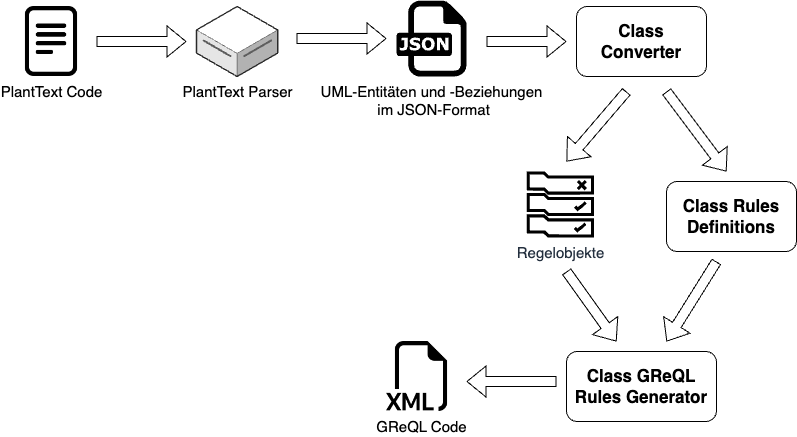
\includegraphics[width=13cm]{images/transit}
    \caption{Schema des Datentransits im GReQL-Converter}
    \label{fig:transit}
\end{figure}

\subsection{Prozess der Integration neuer Regeln}

In diesem Abschnitt wird gezeigt, wie man im Code des GReQL Converters neue Regeln hinzuzufügen kann. Bei der Entwicklung
wurde stets berücksichtigt, dass das Tool weiter verbessert werden muss. Dies beeinflusste den Entwicklungsprozess,
der darauf abzielte, Abstraktionen zu priorisieren, um eine solide Grundlage für die Verbesserung der
Tool-Funktionalitäten zu schaffen.

Ein Entwickler möchte eine Regel hinzufügen, die die Anzahl der Methoden in einer Klasse bestimmt: ``count\_class\_methods''.
Zunächst muss er die Parameter bestimmen, die diese Regel ausmachen, und sie in der Class Rules Definition definieren.
Im Fall von ``count\_class\_methods'' muss er als Attribut den Klassennamen, der untersucht werden soll, sowie die
Anzahl der Methoden haben. Nach dieser Definition muss der Entwickler eine neue PlantText-Annotation im ``Class Converter''
erstellen, um die Identifizierung dieses neuen Regeltyps zu ermöglichen (unter der Annahme, dass die Regel
aus dem PlantText-Code generiert werden soll und nicht manuell). Nach der Entwicklung der Annotation soll eine Methode
in der ``Class Converter'' erstellt werden. Diese Methode wird dazu dienen, ein JSON-Objekt basierend auf der
hinzugefügten Definition in der ``Class Rules Definition'' zu generieren. Gleichzeitig wird die Methode Informationen
aus der Annotation extrahieren und in das generierte Objekt einfügen. Das erzeugte Objekt wird einer Liste von anderen
Regeln hinzugefügt. Darüber hinaus ist es erforderlich, eine Zuordnung zwischen der identifizierten Annotation und der
neu erstellten Methode herzustellen. Um diese Regel für den Lehrer sichtbar und bearbeitbar zu machen, muss er
eine Vue.js-Klasse erstellen, die die grafische Darstellung der Regel darstellt. Abschließend muss er zum ``Class GReQL
Rule Generator'' gehen, um eine neue Regel und eine neue Methode zur Generierung des entsprechenden GReQL-Codes für die
von ihm erstellte neue Regel hinzuzufügen.

Dieser Prozess zur Hinzufügung einer Regel ist für alle Regeln allgemeingültig. Sobald ein Entwickler dies für eine
Regel durchgeführt hat, wird es für andere Entwickler offensichtlich. Der Arbeitsablauf bleibt für fast alle Regeln auf
der Plattform weitgehend gleich.


\subsection{Prozess zur Erweiterung der Kompatibilität mit einer neuen Plattform}

Aktuell ist BOUML die einzige Plattform, die mit dem GReQL Converter kompatibel ist. Die Hinzufügung der Unterstützung
einer neuen Plattform ist jedoch eine Aufgabe, die im GReQL Converter leicht realisierbar ist. Da sich der Regeltyp und
die Parameter nicht ändern, sind keine wesentlichen Änderungen im Code erforderlich. Der Entwickler muss lediglich eine
neue Query zur Vorlage jeder Regel hinzufügen (siehe Code~\ref{lst:example_more_Queries}). Wenn der GReQL Engine eine
Regel auswertet, prüft er lediglich, ob eine der Queries gültig ist. Wenn die Unterstützung einer neuen Plattform
hinzugefügt werden soll, muss der Entwickler nur die Queries der bereits vorhandenen Regeln vervollständigen, die eine
Erweiterung erfordern. Durch diese Methode muss der Entwickler nur an einer einzigen Stelle im Code Änderungen
vornehmen. Der Lehrer muss keine Zielplattform auswählen. Sobald die Unterstützung hinzugefügt und getestet wurde,
kann der Lehrer automatisch GReQL-Code für diese neue Plattform generieren.

\begin{lstlisting}[caption={ Codebeispiel mit mehreren Queries}, label={lst:example_more_Queries}, float=!ht, language=xml]
<rule type="${rule.existence}" points="${rule.points}">
  <!-- Aggregation Regel -->
  <query>
    <!-- Query for BOUML -->
	from x, y : V{Class}, p: V{Property},
        a,b: V{LiteralString} with
	${checkName}
	isDefined(p.aggregation) and
	p.aggregation="composite" and
	x --&gt; V{Property} --&gt; V{Association}
	--&gt; p &lt;-- y and
	report 1 end
  </query>
  <query>
    <!-- Enterprise Architect Query hier schreiben -->
  </query>
  <feedback>${rule.feedback}</feedback>
</rule>
\end{lstlisting}

\subsection{Prozess der Erweiterung um einen neuen Diagrammtypen}


Der GReQL Converter arbeitet nur mit Klassendiagrammen. Es ist jedoch geplant, dass das Tool sich weiterentwickeln kann,
indem es andere Arten von Diagrammen integriert. Um die Unterstützung eines neuen Diagrammtyps hinzuzufügen, muss der
Entwickler zunächst eine Datei ähnlich dem ``Class Converter'' erstellen. Für Sequenzdiagramme könnte dies beispielsweise
``Sequenz Converter'' genannt werden. Es sollte die gleichen Funktionen wie der Class Converter haben, jedoch für
Sequenzdiagramme. Es wird eine Anfrage an den PlantUML-Parser gesendet, der ein Objekt zurückgibt, das die Entitäten
und Beziehungen zwischen den Elementen des Sequenzdiagramms darstellt, das mit PlantText generiert wurde. Anschließend
verwendet der Sequenz Converter eine ``Sequenz Rules Definition''-Datei, um Regeln zu generieren, die auf dem gleichen
Prinzip basieren, das im Abschnitt zum Datentransit im GReQL-Converter beschrieben ist
(siehe Abschnitt~\ref{subsec:datentransit-im-greql-converter}). Danach muss der Entwickler Vue.js-Klassen erstellen, die
zur grafischen Modifikation und Visualisierung jeder dieser Regeln dienen. Abschließend muss der Entwickler einen
``Sequenz GReQL Rules Generator'' erstellen, der den GReQL-Code für jede Regel generiert (basierend auf dem gleichen
Prinzip wie der Class GReQL Rules Generator).

Es ist wichtig zu betonen, dass zusätzliche Änderungen an der Startseite und der Tool-Dokumentation erforderlich sind,
um dem Toolbenutzer zu ermöglichen zu sehen, dass diese Funktionalität bereits möglich ist. Dieser Prozess zur
Hinzufügung eines neuen Diagrammtyps ist generisch. Sobald der Entwickler den Prozess für Klassen verstanden hat, ist es
recht einfach, dasselbe für andere Arten von Diagrammen zu tun. Diese Strategie wurde von Anfang an während der
Entwicklung des Tools konzipiert, um zukünftige Integrationen zu erleichtern.


\section{Erreichte Ergebnisse}

Der GReQL Converter ist ein Instrument zur Generierung von GReQL-Code aus zuvor bereitgestelltem PlantText-Code. Der
vorherige Abschnitt hat im Detail den Prozess der Extraktion von Regeln aus PlantText-Code bis hin zur Generierung
von GReQL-Code beschrieben. Es ist jedoch von entscheidender Bedeutung, die Frage zu beantworten, ob dieses Werkzeug
effektiv funktioniert. Selbst wenn es funktioniert, ist seine Nützlichkeit von Interesse. Im folgenden Kapitel wird
die Frage der Evaluation erörtert. Dabei werden die verschiedenen Prozesse ausführlich beschrieben, die zur Prüfung
des Tools verwendet wurden. Darüber hinaus wird eine gründliche Untersuchung durchgeführt, um die Relevanz dieses
Tools für verschiedene Lehrkräfte nachzuweisen.